\section{Énoncés des Exercices}

\subsection{Suites récurrentes de \texorpdfstring{$\R$}{R}}

% --- Exercice 1 (Source: Exercice 43 analyse) ---
\begin{exercice}[Exercice 43 Analyse]
    Soit $x_{0}\in\R$. On définit la suite $(u_{n})$ par $u_{0}=x_{0}$ et, $\forall n\in\N$, $u_{n+1}=\arctan(u_{n}).$
    \begin{enumerate}
        \item 
        \begin{enumerate}
            \item Démontrer que la suite $(u_{n})$ est monotone et déterminer, en fonction de la valeur de $x_{0}$, le sens de variation de $(u_{n})$.
            \item Montrer que $(u_{n})$ converge et déterminer sa limite.
        \end{enumerate}
        \item Déterminer l'ensemble des fonctions $h$ continues sur $\R$ telles que $\forall x\in\R$, $h(x)=h(\arctan x)$.
    \end{enumerate}
\end{exercice}

% --- Exercice 2 (Source: Exercice 1 Suites Arithmético-géométriques) ---
\begin{exercice}
\begin{enumerate}
    \item On considère $a, b\in\R^{*}$, $u_{0}\in\R$ et $(u_{n})$ définie par $\forall n\in\N$, $u_{n+1}=au_{n}+b$.

    Déterminer $u_{n}$ en fonction de $n$.
    \textit{On pourra remarquer que pour un choix judicieux de $c$, la suite $u_{n}-c$ est géométrique.}

    \item 
        Votre banquier préféré vous prête une somme $S$ au taux d'intérêt fixe mensuel de $t\%$ sur une durée de $N$ mois avec remboursement mensuel constant.

        Déterminer votre remboursement mensuel en fonction de $S, t, N$.
\end{enumerate}
\end{exercice}

% --- Exercice 3 (Source: Exercice 2) ---
\begin{exercice}
    On suppose que $f\in \mathscr C^{1}(I,I)$ et que $a\in I$ vérifie $f(a)=a$.
    On considère $u_{0}\in I$ et $\forall n\in\N$, $u_{n+1}=f(u_{n})$.
    On suppose que $f^{\prime}(a)\in]-1,1[$. \\

    Montrer qu'il existe un intervalle $J\subset I$ différent de $\{a\}$ tel que si on suppose $u_{0}\in J$,
    $(u_n)$ converge vers $a$ ($a$ est alors appelé point fixe attractif).
\end{exercice}

% --- Exercice 4 (Source: Exercice 3) ---
\begin{exercice}
    On pose $u_{0}\in\R$ et $u_{n+1}=\frac{1}{3}(u_{n}^{3}+2)$.
    Étudier le comportement de $u_{n}$ en fonction de $u_{0}$.
    Déterminer un développement asymptotique de $u_{n}$ lorsqu'il y a convergence.

    \textit{Pour cela, on posera $v_{n}=1-u_{n}$, on trouvera un réel $\alpha<0$ tel que $v_{n+1}^{\alpha}-v_{n}^{\alpha}$ possède une limite finie non nulle, 
    puis on appliquera le théorème de Cesàro à la suite $v_{n+1}^{\alpha}-v_{n}^{\alpha}$.}
\end{exercice}

% --- Exercice 5 (Source: Exercice 4) ---
\begin{exercice}
    On pose $\alpha=e^{\frac 1 e}$ et on définit une suite $(u_{n})$ par :
    $u_{0}=1$ et $\forall n\in\N$, $u_{n+1}=\alpha^{u_{n}}$.

    Étudier la convergence de cette suite.
\end{exercice}

\newpage
\subsection{Autres suites numériques}
% --- Exercice 6 (Source: EXERCICE 1 analyse) ---
\begin{exercice}[Exercice 1 Analyse]
\begin{enumerate}
    \item On considère deux suites numériques $(u_{n})$ et $(v_{n})$ 
        telles que $(v_{n})_{n\in\N}$ est non nulle à partir d'un certain rang et $u_{n}\sim v_{n}$.
        
        Démontrer que $u_{n}$ et $v_{n}$ sont de même signe à partir d'un certain rang.

    \item Déterminer le signe, au voisinage de l'infini, de $u_{n}=\sinh\left(\frac{1}{n}\right)-\tan\left(\frac{1}{n}\right)$.
\end{enumerate}
\end{exercice}

% --- Exercice 7 (Source: Exercice 5) ---
\begin{exercice}
On pose pour tout naturel $n\geqslant1$, $f_{n}(x)=nx^{n+1}-(n+1)x^{n}-\frac{1}{2}$.
\begin{enumerate}
    \item Montrer qu'il existe un unique réel $x_{n}>0$ tel que $f_{n}(x_{n})=0$.
    \item Montrer que la suite $(x_{n})_{n\in\N}$ est monotone et qu'elle converge.
    \item Déterminer sa limite $\ell$.
    \item Déterminer un équivalent de $x_{n}-\ell$.

    \textit{Indication : On montrera d'abord qu'il existe un unique réel $\alpha>0$ tel que $e^{\alpha}(\alpha-1)=\frac{1}{2}$. 
    On calculera ensuite pour $\beta\in\R$ un équivalent de $f_{n}\left(1+\frac{\alpha}{n}+\frac{\beta}{n^{2}}\right)$. 
    On en déduira qu'il existe deux réels $\beta$ et $\beta^{\prime}$ tels que pour $n$ assez grand 
    $1+\frac{\alpha}{n}+\frac{\beta}{n^{2}}\leqslant x_{n}\leqslant 1+\frac{\alpha}{n}+\frac{\beta^{\prime}}{n^{2}}$ puis on conclura.}
\end{enumerate}
\end{exercice}

% --- Exercice 8 (Source: Exercice 6) ---
\begin{exercice}
    Soit $(x_{n})$ une suite réelle. Définissons les suites $(y_{n})$ et $(z_{n})$ par :
    $\forall n\in\N^{*}$, $y_{n}=x_{n+1}-x_{n}$ et $z_{n}=\frac{x_{n}}{n}$.

    Montrer que si $\lim_{n \to + \infty} y_{n} = \ell$ alors $\lim_{n \to + \infty} z_{n} = \ell$.
    Trouver un contre-exemple à la réciproque.
\end{exercice}

\subsection{Suites d'un espace vectoriel normé}
% --- Exercice 9 (Source: Exercice 7) ---
\begin{exercice}
    On se place dans l'espace des fonctions bornées de $\R^{+}$ dans $\R$ muni de la norme infinie.
    Étudier la convergence de la suite $(f_{n})$ de fonctions dans les cas suivants :
    \begin{enumerate}
        \item $f_{n}:\R^{+}\rightarrow\R, \quad x\mapsto\frac{x}{1+nx}$
        \item $f_{n}:\R^{+}\rightarrow\R, \quad x\mapsto nxe^{-nx}\sin(x)$
        \item $f_{n}:\R^{+}\rightarrow\R, \quad x\mapsto\frac{ne^{-x}+1}{x^{2}+n}$
    \end{enumerate}
    \textit{On commencera par démontrer que si $f_{n}$ converge vers $f$ pour la norme $\|\cdot\|_{\infty}$ alors pour tout $x$, $f_{n}(x)$ converge vers $f(x)$.}
\end{exercice}

% --- Exercice 10 (Source: Exercice 8) ---
\begin{exercice}
    On se place dans l'espace $E=\ell^{\infty}(\R)$ des suites bornées sur $\R$ muni de la norme infinie.

    On considère une suite $(X_{p})$ d'éléments de $E$ définie par : 
    $\forall p\in\N, X_{p}=(u_{n,p})_{n}$ avec $u_{n,p}=1$ si $n<p$ et $0$ sinon.

    On suppose dans un premier temps que la suite $(X_{p})$ converge vers une suite $Y=(y_{n})_{n\in\N}$.

    Montrer qu'alors pour tout naturel $n$, $y_{n}$ est la limite quand $p$ tend vers l'infini de la suite $u_{n,p}$.
    
    En déduire la valeur de $Y$. Conclure.
\end{exercice}

% --- Exercice 11 (Source: Exercice 9) ---
\begin{exercice}
    On munit $\mathscr M_{p}(\R)$ de la norme $N(A) = \max\{|a_{ij}|, i,j\in\{1,\dots,p\}\}$.
    Soit $A\in \mathscr M_{p}(\R)$ telle que la suite $A^{n}$ converge.

    Montrer que la limite $L$ de la suite vérifie $L^{2}=L$. Qu'en déduire ?
\end{exercice}

\subsection{Valeurs d'adhérence}
% --- Exercice 12 (Source: Exercice 10) ---
\begin{exercice}
    Soit $(x_{n})$ une suite réelle bornée. On pose pour tout naturel $n$,
    $a_{n}=\inf\{x_{p},p\geqslant n\}$ et $b_{n}=\sup\{x_{p},p\geqslant n\}$.
    \begin{enumerate}
        \item Montrer que ces deux suites sont monotones et bornées.
        \item On note $\ell$ la limite de la suite $(a_{n})$.
        
            Montrer que $\ell$ est une valeur d'adhérence de la suite $(x_{n})$.
            Quel théorème venons-nous de démontrer ?
    \end{enumerate}
\end{exercice}

% --- Exercice 13 (Source: Exercice 11) ---
\begin{exercice}
    Soit $(a_{n})$ une suite réelle telle que $a_{n+1}-a_{n}$ tend vers 0.
    Montrer que l'ensemble des valeurs d'adhérence de cette suite est un intervalle.
\end{exercice}

% --- Exercice 14 (Source: Exercice 12) ---
\begin{exercice}
    On considère une suite $(u_{n})$ de réels strictement positifs tels que $\forall n,p\in\N$, $u_{n+p}\leqslant u_{n}+u_{p}$ 
    et on pose pour tout naturel $n$, $x_{n}=\frac{u_{n}}{n}$.
    \begin{enumerate}
        \item Montrer que la suite $(x_{n})_{n\in\N}$ est bornée.
        \item En déduire que l'on peut définir pour tout naturel $n$, $y_{n}=\sup\{x_{p}, p\geqslant n\}$.
        \item Montrer que la suite $y_{n}$ converge. On notera $\ell$ sa limite.
        \item Montrer que $\ell$ est une valeur d'adhérence de $(x_{n})$.
        \item On fixe un entier $q$ non nul, montrer en utilisant la division euclidienne de $n$ par $q$ qu'il existe une constante $M_{q}$ 
            telle que pour tout naturel $n$, $x_{n}\leqslant x_{q}+\frac{M_{q}}{n}$.
        \item En déduire que pour tout $q$ naturel, $\ell\leqslant x_{q}$ et enfin que la suite $(x_{n})_{n\in\N}$ converge vers $\ell$.
    \end{enumerate}
    \textit{Ce résultat s'appelle le lemme sous-additif ou lemme de Fekete.}
\end{exercice}

\newpage
\section{Corrections}

% --- Correction 1 ---
\begin{correction}{1}
On pose $f(x)=\arctan x$.

\begin{enumerate}
\item~
    \begin{enumerate}
        \item
        \textit{Premier cas : Si $u_{1}<u_{0}$.}
        Puisque la fonction $f:x\mapsto \arctan x$ est strictement croissante sur $\R$, alors $\arctan(u_{1})<\arctan(u_{0})$, c'est-à-dire $u_{2}<u_{1}$.
        Par récurrence, on prouve que $\forall n\in\N$, $u_{n+1}<u_{n}$. Donc la suite $(u_{n})$ est strictement décroissante.

        \textit{Deuxième cas : Si $u_{1}>u_{0}$.}
        Par un raisonnement similaire, on prouve que la suite $(u_{n})$ est strictement croissante.

        \textit{Troisième cas : Si $u_{1}=u_{0}$.}
        La suite $(u_{n})$ est constante.

        Pour connaître les variations de la suite $(u_{n})$ il faut donc déterminer le signe de $u_{1}-u_{0}$, signe de $\arctan(u_{0})-u_{0}$.
        On pose alors $g(x)=\arctan x - x$ et on étudie le signe de la fonction $g$.
        On a $\forall x\in\R$, $g^{\prime}(x)=\frac{1}{1+x^{2}} - 1 = \frac{-x^{2}}{1+x^{2}}$ et donc $\forall x\in\R^{*}$, $g^{\prime}(x)<0$.
        Donc $g$ est strictement décroissante sur $\R$ et comme $g(0)=0$ alors :
        $\forall x\in]0,+\infty[$, $g(x)<0$ et $\forall x\in]-\infty,0[$, $g(x)>0$.
        On a donc trois cas suivant le signe de $x_{0}$ :
        \begin{itemize}
            \item Si $x_{0}>0$, la suite $(u_{n})$ est strictement décroissante.
            \item Si $x_{0}=0$, la suite $(u_{n})$ est constante.
            \item Si $x_{0}<0$, la suite $(u_{n})$ est strictement croissante.
        \end{itemize}

        \item 
        La fonction $g$ étant strictement décroissante et continue sur $\R$, elle induit une bijection de $\R$ sur $g(\R)=\R$.
        
        $0$ admet donc un unique antécédent par $g$ et, comme $g(0)=0$, alors 0 est le seul point fixe de $f$.
        Donc si la suite $(u_{n})$ converge, elle converge vers 0, le seul point fixe de $f$.
        \begin{itemize}
            \item \textit{Si $u_{0}>0$ :} L'intervalle $]0,+\infty[$ étant stable par $f$, on a par récurrence $\forall n\in\N, u_{n}>0$. 
                Donc la suite $(u_{n})$ est décroissante et minorée par 0, donc elle converge vers 0, unique point fixe de $f$.
            \item \textit{Si $u_{0}<0$ :} Par un raisonnement similaire, on prouve que $(u_{n})$ est croissante et majorée par 0, donc elle converge vers 0.
            \item \textit{Si $u_{0}=0$ :} La suite est constante égale à 0.
        \end{itemize}

        \textit{Conclusion :} $\forall u_{0}\in\R$, $(u_{n})$ converge vers 0.
    \end{enumerate}

    \item 
    Soit $h$ une fonction continue sur $\R$ telle que $\forall x\in\R, h(x)=h(\arctan x)$.
    Soit $x\in\R$. 

    Considérons la suite $(u_{n})$ définie par $u_{0}=x$ et $u_{n+1}=\arctan(u_{n})$.

    On a alors $h(x)=h(u_{0})=h(\arctan(u_{0}))=h(u_{1})=h(\arctan(u_{1}))=h(u_{2})=\dots$

    Par récurrence, on prouve que $\forall n\in\N$, $h(x)=h(u_{n})$.

    De plus, par convergence de la suite $(u_{n})$ vers 0 et par continuité de $h$, $\lim_{n\rightarrow+\infty}h(u_{n})=h(0)$ 

    On obtient ainsi : $h(x)=h(0)$ et donc $h$ est une fonction constante.

    Réciproquement, toutes les fonctions constantes conviennent.
\end{enumerate}
\end{correction}

% --- Correction 2 ---
\begin{correction}{2}
\begin{enumerate}
    \item 
    On pose $c$ la constante telle que $c=ac+b$, c'est-à-dire $c=\frac{b}{1-a}$.

    Alors $v_{n}=u_{n}-c$ est géométrique de raison $a$.

    Donc pour tout $n$, $v_{n}=a^{n}v_{0}$ donc $u_{n}=c+a^{n}(u_{0}-c)$.

    \item 
    On note $u_{n}$ le capital restant dû au bout de $n$ mois.

    On a donc $u_{0}=S$, pour tout $n$, $u_{n+1}=(1+t)u_{n}-R$.

    D'après la question pécédente : $u_n = \frac{R}{t} + (1+t)^n(S - \frac{R}{t})$

    De plus $u_N = 0$, d'où :
    \begin{align*}
        0 &= \frac{R}{t} + (1+t)^N(S-\frac{R}{t})\\
        \iff R &= (1+t)^N(R-t\cdot S)\\
        \iff R &= -\frac{t\cdot S(1+t)^N}{1-(1+t)^N}
    \end{align*}
\end{enumerate}
\end{correction}

% --- Correction 3 ---
\begin{correction}{3}

    Par continuité de $f'$, il existe $\alpha>0$ et $\beta\in]0,1[$ tels que $\forall x\in]a-\alpha,a+\alpha[, |f^{\prime}(x)|\leqslant\beta$. \\
    Posons $J=]a-\alpha,a+\alpha[\cap I$. \\
    Tout d'abord $J$ est bien stable par $f$, car si $x\in J$, $x\in I$ donc $f(x)\in I$.

    De plus par l'inégalité des accroissements finis, \\
    $|f(x)-a|=|f(x)-f(a)|\leqslant \sup_{[a,x]}|f^{\prime}|\cdot|x-a|\leqslant\beta|x-a| < |x-a| \leqslant \alpha$. Donc $f(x)\in J$. \\

    Ainsi si on pose $u_{0}\in J$ tous les $u_{n}$ sont dans $J$. \\
    Et donc toujours par l'inégalité des accroissements finis, pour tout $n$, $|u_{n+1}-a|=|f(u_{n})-f(a)|\leqslant\beta|u_{n}-a|$. \\
    Et donc par récurrence $|u_{n}-a|\leqslant\beta^{n}|u_{0}-a|$ qui converge vers 0. \\

    Conclusion : $(u_n)$ converge vers $a$.
\end{correction}

% --- Correction 4 ---
\begin{correction}{4}

    On pose pour $x$ réel $f(x)=\frac{1}{3}(x^{3}+2)$ et $g(x)=f(x)-x$. \\
    $f$ et $g$ sont polynomiales donc $C^{1}$ et pour tout $x$, $f^{\prime}(x)=x^{2}$ et $g^{\prime}(x)=x^{2}-1$.

    On étudie les variations :

    \begin{tikzpicture}
    \tkzTabInit[lgt=2, espcl=3] 
      {$x$ / 1, $g'(x)$ / 1, $g(x)$ / 2} 
      {$-\infty$, $-1$, $1$, $+\infty$}
  
    \tkzTabLine{, +, z, -, z, +, }

    \tkzTabVar{-/ $-\infty$, +/ $\frac{4}{3}$, -/ $0$, +/ $+\infty$}
    \tkzTabVal{1}{2}{0.5}{-2}{0}
    \end{tikzpicture}
   
    On remarque que les seuls points fixes de $f$ sont $-2$ et $1$. \\
    On en déduit que :
    \begin{itemize}
        \item Si $u_{0}\in\{-2,1\}$, la suite est constante.
        \item Si $u_{0}\in]-\infty,-2[$, comme cet intervalle est stable, tous les $u_{n}$ y sont, \\
            donc $u_{n+1}-u_{n}=g(u_{n})\leqslant0$, donc la suite est décroissante. \\
            Si elle était convergente, elle convergerait vers un point fixe $l$ avec $l\leqslant u_{0}<-2$, absurde. \\
            Donc elle diverge vers $-\infty$.
        \item Si $u_{0}\in]-2,1[$, comme cet intervalle est stable, $u_{n+1}-u_{n}=g(u_{n})\geqslant0$,
            donc la suite est croissante. \\
            Elle est majorée par 1, donc converge vers un point fixe $l$ avec $-2<u_{0}\leqslant l\leqslant1$, donc $l=1$.
        \item Si $u_{0}\in]1,+\infty[$, intervalle stable, $u_{n+1}-u_{n}\geqslant0$, suite croissante. \\
            Si elle était conergente, elle convergerait vers $l \geqslant u_0 > 1$, absurde. Elle diverge vers $+\infty$.
    \end{itemize}
    Les cas de convergence sont donc $u_{0}\in\{-2,1\}$ où la suite est constante et $u_{0}\in]-2,1[$. \\
    Dans ce dernier cas on pose $v_{n}=1-u_{n}$ qui est positive et converge vers 0.
    
    On trouve ensuite une relation de récurrence entre $v_{n+1}$ et $v_{n}$. 

    \begin{align*}
        v_{n+1} &= 1-u_{n+1}\\
        &= 1-\frac{u_n^3+2}{3}\\
        &=1-\frac{(1-v_n)^3+2}{3}\\
        &=\frac{1-(1-v_n)^3}{3}\\
        &= v_n - v_n^2 + \frac{1}{3} v_n^3\\
        &= v_n \cdot \left(1 - v_n +\frac{1}{3}v_n^2\right)
    \end{align*}

    Ainsi pour $\alpha < 0$ :
    \begin{align*}
        v_{n+1}^\alpha &= v_n^\alpha\cdot\left(1-v_n+\frac{1}{3}v_n^2\right)^\alpha\\
        &= v_n^\alpha\cdot\left(1-v_n+o(v_n)\right)^\alpha\\
        &= v_n^\alpha - \alpha \cdot v_n^{\alpha+1} +o\left(v_n^{\alpha+1}\right)
   \end{align*}

Et donc :
\[v_{n+1}^\alpha - v_n^\alpha \sim -\alpha\cdot v_n^{\alpha+1}\]
A une limite non nul pour $\alpha = -1$ dans ce cas la limite est $1$.

En applicant le théoreme de Cesàro $$ \frac{1}{n}\sum_{k=0}^{n-1}v_{k+1}^{-1} - v_k^{-1} = \frac{v_n^{-1}-v_0^{-1}}{n} \xrightarrow[n\to\infty]{} 1 $$

Donc $ v_n \sim \frac{1}{n}$
Finalement :
\[u_n = 1-v_n = 1 -\frac{1}{n}+o\left(\frac{1}{n}\right)\]
\end{correction}

\newpage
% --- Correction 5 ---
\begin{correction}{5}

Pour pouvoir poser $f(x)=\alpha^{x}=e^{x \ln \alpha}=e^{\frac{x}{e}}$.

On vérifie aisément que $[0,e]$ est stable par $f$.

On étudie la fonction $f$, la fonction $g$ définie par $g(x)=f(x)-x$.

Pour $x\in\R_+^*$ : $ g'(x) = \frac{1}{e}e^{\frac{x}{e}}-1$


\begin{tikzpicture}
    \tkzTabInit[lgt=2,espcl=3]
        {$x$ / 1, $g'(x)$ / 1, $g(x)$ / 2} 
        {$0$, $e$,  $+\infty$}

    \tkzTabLine{, -, z, +, }

    \tkzTabVar{+/ $1$, -/ $0$, +/ $+\infty$}
\end{tikzpicture}

On trace le tableau de variation et on en déduit que $e$ est l'unique point fixe de $f$ et que $(u_n)$ est croissante.
Donc $u_n \to e$.
\end{correction}

% --- Correction 6 ---
\begin{correction}{6}
\begin{enumerate}
    \item 
    Par hypothèse, $\exists N_{0}\in\N, \forall n\geqslant N_{0}, v_{n}\ne0$. \\
    Ainsi la suite $\left(\frac{u_{n}}{v_{n}}\right)$ est définie à partir du rang $N_{0}$. \\
    Comme $u_{n}\sim v_{n}$, on a $\lim_{n\rightarrow+\infty}\frac{u_{n}}{v_{n}}=1$. \\
    Alors, $\forall\varepsilon>0, \exists N\geqslant N_{0}, \forall n\geqslant N \Rightarrow |\frac{u_{n}}{v_{n}}-1|\leqslant\varepsilon$. \\
    Prenons $\varepsilon=\frac{1}{2}$. On en déduit que pour $n \geqslant N$, $\frac{1}{2} \leqslant \frac{u_n}{v_n} \leqslant \frac{3}{2}$. \\
    Donc $\frac{u_{n}}{v_{n}}>0$, ce qui implique que $u_{n}$ et $v_{n}$ sont de même signe.

    \item
    Au voisinage de $+\infty$, $\sinh\left(\frac{1}{n}\right)=\frac{1}{n}+\frac{1}{6n^{3}}+o\left(\frac{1}{n^{3}}\right)$
    et $\tan\frac{1}{n}=\frac{1}{n}+\frac{1}{3n^{3}}+o(\frac{1}{n^{3}})$. \\
    Donc $u_{n}\sim -\frac{1}{6n^{3}}$. \\
    On en déduit, d'après 1, qu'à partir d'un certain rang, $u_{n}$ est négatif.
\end{enumerate}
\end{correction}

% --- Correction 7 ---
\begin{correction}{7}
\begin{enumerate}

    \item Etudions $f_n$ :

    Pour $x\in\R_+$ : $f_n'(x) = n(n+1)\left(x^n -x^{n-1}\right)$

    \begin{tikzpicture}
        \tkzTabInit[lgt=2,espcl=3]
            {$x$ / 1, $f'(x)$ / 1, $f(x)$ / 2} 
            {$0$, $1$,  $+\infty$}

        \tkzTabLine{ z, - ,z, +, }

        \tkzTabVar{+/ $-\frac{1}{2}$, -/ $-\frac{3}{2}$, +/ $+\infty$}
        \tkzTabVal{2}{3}{0.5}{$x_n$}{0}
    \end{tikzpicture}

    $x_n$ existe et est unique par le théorème de la bijection.
    
    \item La stricte croissance de $f_{n}$ montre que $x_{n+1}-x_{n}$ 
        est du même signe que $f_{n}(x_{n+1})-f_{n}(x_{n})=f_{n}(x_{n+1})$ car $f_n(x_n)=0$. \\
        Or $f_{n+1}(x_{n+1})=0=(n+1)x_{n+1}^{n+2}-(n+2)x_{n+1}^{n+1}-\frac{1}{2}$.
        Donc $\frac{1}{2}=(n+1)x_{n+1}^{n+2}-(n+2)x_{n+1}^{n+1}$. \\
        En injectant dans $f_n(x_{n+1})$, on trouve que $f_{n}(x_{n+1}) \leqslant 0$ après factorisation. \\
        Donc la suite décroît et est minorée par 1.

        Elle converge.

    \item On a $\ell\ge1$. Supposons par l'absurde que $\ell>1$.  \\

    Pour tout $n\in\N$ :
    \begin{align*}
        f_{n}(x_n)=nx_n^{n+1}-(n+1)x_n^{n}-\frac{1}{2} &= 0 \\
        \text{Donc : } x_n^n (nx_n - (n+1)) &= \frac{1}{2} 
    \end{align*}
    Donc : $ nx_n - (n+1) \sim \frac{1}{2\ell}$

    Or : $ nx_n - (n+1) = n(x_n-1) + 1 \sim n(x_n-1) \to+\infty \neq \frac{1}{2\ell}$ ce qui est contradictoire

    Finalement $\ell=1$ 

    \item \textbf{Existence de $\alpha$ :} 

    Posons $\varphi(t) = e^t(t-1)$. La fonction $\varphi$ est dérivable sur $\R$ et $\varphi'(t) = e^t(t-1) + e^t = te^t$. 

    Pour $t > 0$, $\varphi'(t) > 0$, donc $\varphi$ est strictement croissante sur $\R_+^*$. 

    De plus, $\varphi(0) = -1$ et $\lim_{t \to +\infty} \varphi(t) = +\infty$. 

    Comme $\varphi$ est continue et strictement croissante, elle réalise une bijection de $\R_+^*$ sur $]-1, +\infty[$. 

    Puisque $\frac{1}{2} \in ]-1, +\infty[$, il existe un unique réel $\alpha > 0$ tel que $\varphi(\alpha) = \frac{1}{2}$, soit $e^\alpha(\alpha - 1) = \frac{1}{2}$.


    \textbf{Équivalent de $f_n\left(1 + \frac{\alpha}{n} + \frac{\beta}{n^2}\right)$ :}

    Posons $u_n = 1 + \frac{\alpha}{n} + \frac{\beta}{n^2}$. Exprimons $f_n(u_n)$ :
    $$f_n(u_n) = n u_n^{n+1} - (n+1)u_n^n - \frac{1}{2} = u_n^n (nu_n - n - 1) - \frac{1}{2}$$

    D'une part, $nu_n - n - 1 = n\left(1 + \frac{\alpha}{n} + \frac{\beta}{n^2}\right) - n - 1 = \alpha - 1 + \frac{\beta}{n}$.
    
    D'autre part, effectuons un développement asymptotique de $u_n^n = \exp(n \ln(u_n))$ :
    \begin{align*}
        \ln(u_n) &= \ln\left(1 + \frac{\alpha}{n} + \frac{\beta}{n^2}\right) \\
        &= \frac{\alpha}{n} + \frac{\beta}{n^2} - \frac{1}{2}\left(\frac{\alpha}{n}\right)^2 + o\left(\frac{1}{n^2}\right) \\
        &= \frac{\alpha}{n} + \frac{\beta - \frac{\alpha^2}{2}}{n^2} + o\left(\frac{1}{n^2}\right)
    \end{align*}
    Donc, $n \ln(u_n) = \alpha + \frac{\beta - \frac{\alpha^2}{2}}{n} + o\left(\frac{1}{n}\right)$.

    En passant à l'exponentielle :
    \begin{align*}
        u_n^n &= e^\alpha \exp\left(\frac{\beta - \frac{\alpha^2}{2}}{n} + o\left(\frac{1}{n}\right)\right) \\
        &= e^\alpha \left( 1 + \frac{\beta - \frac{\alpha^2}{2}}{n} + o\left(\frac{1}{n}\right) \right)
    \end{align*}
    
    On remplace dans l'expression de $f_n(u_n)$ :
    \begin{align*}
        f_n(u_n) &= e^\alpha \left( 1 + \frac{\beta - \frac{\alpha^2}{2}}{n} + o\left(\frac{1}{n}\right) \right) \left( \alpha - 1 + \frac{\beta}{n} \right) - \frac{1}{2} \\
        &= e^\alpha \left( (\alpha - 1) + \frac{\beta}{n} + \frac{(\alpha - 1)\left(\beta - \frac{\alpha^2}{2}\right)}{n} \right) - \frac{1}{2} + o\left(\frac{1}{n}\right) \\
        &= e^\alpha (\alpha - 1) + \frac{e^\alpha}{n} \left( \beta + (\alpha - 1)\beta - \frac{\alpha^2(\alpha - 1)}{2} \right) - \frac{1}{2} + o\left(\frac{1}{n}\right)
    \end{align*}

    Or, par définition de $\alpha$, $e^\alpha(\alpha - 1) = \frac{1}{2}$ :
    $$f_n(u_n) = \frac{e^\alpha}{n} \left( \alpha\beta - \frac{\alpha^2(\alpha - 1)}{2} \right) + o\left(\frac{1}{n}\right)$$

    Ainsi, on obtient l'équivalent suivant (pourvu que la parenthèse soit non nulle) :
    $$f_n\left(1 + \frac{\alpha}{n} + \frac{\beta}{n^2}\right) \sim \frac{e^\alpha}{n} \left( \alpha\beta - \frac{\alpha^2(\alpha - 1)}{2} \right)$$
    
    \textbf{Conclusion :}

    Le signe de $f_n\left(1 + \frac{\alpha}{n} + \frac{\beta}{n^2}\right)$ pour $n$ assez grand est donné par le signe de $\alpha\beta - \frac{\alpha^2(\alpha - 1)}{2}$.

    Puisque $\alpha > 0$, l'expression $\alpha\beta - \frac{\alpha^2(\alpha - 1)}{2}$ est strictement croissante en fonction de $\beta$.
    \begin{itemize}
        \item En choisissant un réel $\beta$ suffisamment petit (par exemple négatif), cette quantité est strictement négative. Pour un tel $\beta$, $f_n\left(1 + \frac{\alpha}{n} + \frac{\beta}{n^2}\right) < 0$ pour $n$ assez grand.
        \item En choisissant un réel $\beta'$ suffisamment grand, cette quantité est strictement positive. Pour un tel $\beta'$, $f_n\left(1 + \frac{\alpha}{n} + \frac{\beta'}{n^2}\right) > 0$ pour $n$ assez grand.
    \end{itemize}

    Or, par définition $f_n(x_n) = 0$. Comme $f_n$ est strictement croissante sur $[1, +\infty[$ et que les termes considérés sont supérieurs à 1, on a :
    $$f_n\left(1 + \frac{\alpha}{n} + \frac{\beta}{n^2}\right) \leqslant f_n(x_n) \leqslant f_n\left(1 + \frac{\alpha}{n} + \frac{\beta'}{n^2}\right)$$

    qui donne :
    $$1 + \frac{\alpha}{n} + \frac{\beta}{n^2} \leqslant x_n \leqslant 1 + \frac{\alpha}{n} + \frac{\beta'}{n^2}$$

    On retranche la limite $\ell = 1$ et on multiplie par $n$ :
    $$\alpha + \frac{\beta}{n} \leqslant n(x_n - 1) \leqslant \alpha + \frac{\beta'}{n}$$

    D'après le théorème des gendarmes, on en déduit que $\lim_{n \to +\infty} n(x_n - 1) = \alpha$.
    En conclusion, puisque $\alpha \neq 0$ :
    $$x_n - \ell \sim \frac{\alpha}{n}$$
\end{enumerate}
\end{correction}

% --- Correction 8 ---
\begin{correction}{8}

On applique le théorème de Cesàro à la suite $y_{n}$.
$$z_n = \frac{1}{n} \sum_{k=0}^{n-1} (x_{k+1}-x_k) + \frac{x_0}{n} = \frac{1}{n} \sum_{k=0}^{n-1} y_k + \frac{x_0}{n}$$

La moyenne de Cesàro converge vers $\ell$, et le terme $x_0/n$ tend vers 0. Donc $(z_n)$ tend vers $\ell$.

$(-1)^n$ ou $\mathbb{sin}(\frac{\pi}2 n)$ sont des contre-exemples à la réciproque ($z_n \to 0$ mais $y_n$ ne converge pas).
\end{correction}

\begin{correction}{9}

\uline{Démonstration du lemme :}

Supposons que $f_n \xrightarrow[n\to+\infty]{||\cdot||_{\infty}} f \in E$, c'est à dire que $(f_n)$ converge uniformément vers f.

Alors pour $x \in \R^{+}$ fixé, $|f_n(x) - f(x)| \leqslant ||f_n - f||_{\infty}$ or $||f_n - f||_{\infty} \rightarrow 0$

Donc $f_n(x) - f(x) \rightarrow 0$ donc $f_n(x) \rightarrow f(x)$.

On dit que "$f_n$ converge simplement vers f".\\

\uline{Questions :}
\begin{enumerate}
    \item~
    \begin{itemize}
        \item Étude de la convergence simple :

        Si $x = 0$, $f_n(x) = 0 \rightarrow 0$.

        Si $x \not \equal 0$, $f_n(x) \sim \frac{x}{nx} = \frac 1 n \rightarrow 0$

        \item Étude de la convergence uniforme :

        $f_n$ est $C^1$ par théorèmes d'opérations.

        $\forall x, f_n'(x) = \frac{1 + nx - nx}{(1 + nx)^2} = \frac 1 {(1 + nx)^2}$

        Donc $f_n$ est strictement croissante,
        
        Donc $\norm{f_n}_\infty = \ds\lim_{x\to+\infty}f_n(x) = \frac{1}{n}$

        Donc $||f_n||_{\infty} \rightarrow 0$.

        Ainsi $(f_n)$ converge simplement et uniformément vers la fonction nulle sur $\R_+$
    \end{itemize}

    \item~
    \begin{itemize}
        \item Convergence simple :

        Pour tout $x\in\R_+$ : $ f_n(x)\xrightarrow[n\to+\infty]{} 0$ par croissances comparées.
        
        \item Convergence uniforme :

        Pour $x\in\R_+$ : $f(x) \leqslant \underbrace{nx^2e^{-nx}}_{g_n(x)} $  (car sur $\R_+, \sin(x) \leqslant x$)

        Et : $g'_n(x) = nx(2-nx)e^{-nx}$

        \begin{tikzpicture}
            \tkzTabInit[lgt=2,espcl=3]
                {$x$ / 1,$g'(x)$ / 1,$g(x)$ / 2.5}
                {$0$ , $\frac{2}{n}$ , $+\infty$}

            \tkzTabLine{,+,z,-,}

            \tkzTabVar{-/ $0$, +/ $\frac{4}{ne^2}$, -/ $0$}
        \end{tikzpicture}

        Ainsi : $\forall x\in\R_+, f_n(x) \leqslant \frac{4}{ne^2}$

        Donc : $\norm{f_n}_\infty \to 0$        


        Finalement : $(f_n)$ converge simplement et uniformément vers la fonction nulle sur $\R_+$
    \end{itemize}
    
    \item~
    \begin{itemize}
        \item Convergence simple :

        $\forall x\in\R_+, f_n(x)\xrightarrow[n\to+\infty]{} e^{-x}$
        \item Convergence uniforme :

        $\forall x\in\R_+, \abs{f_n(x)-e^{-x}} = f_n(x)-e^{-x} \leqslant \frac{1}{n}$

        Donc $\norm{f_n}_\infty \to 0$

        Finalement $(f_n)$ converge simplement et uniformément vers $\fonction{f}{\R_+}{\R}{x}{e^{-x}}$
    \end{itemize}
\end{enumerate}    
\end{correction}

\begin{correction}{10}

    \uline{\textbf{Analyse :}}
    
    Supposons que $(X_p)$ converge vers une suite $Y$.
       
    Alors, $\norm{X_p - Y} \to 0$

    C'est à dire $\ds\sup_{k\in\N}\{x_{k,p}-y_k\} \to 0$

    Or : $\forall n\in\N, \abs{x_{n,p} - y_n } \leqslant \ds\sup_{k\in\N}\{x_{k,p}-y_k\} \to 0 $

    Et : $x_{n,p} \xrightarrow[p\to+\infty]{} 1 $

    D'où : $Y$ est la suite constante égale à 1.

    \uline{\textbf{Synthese :}}

    Soit $Y = (1)_{n\in\N}$

    $\norm{X_p-Y} = \ds\sup_{k\in\N}\{x_{k,p} - 1\} = 1 \not\to 0$

    Donc $(X_p)$ ne converge pas vers $Y$ donc d'après l'analyse $(X_p)$ ne converge pas pour $\norm{\cdot}$
\end{correction}


\begin{correction}{11} \\
On prend la suite $(A^{2n})$ or $A^{2n} = (A^n)^2$ et $M \mapsto M^2$ est continue. Donc $A^{2n} \rightarrow L^2$.
\end{correction}

\begin{correction}{12}
\begin{enumerate}
    \item $\forall n \in \N, a_0 = m \leqslant x_n \leqslant M = b_0$\\
    
    $a_n$ existe car l'ensemble est non vide et minoré donc $a_0 \leqslant a_n \leqslant x_n \leqslant b_0$. Donc $a_n$ bornée.

    On a que $\{x_p \mid p \geqslant n + 1\} \subset \{x_p \mid p \geqslant n\}$. Donc $a_{n+1} \geqslant a_n$. 
    Donc $(a_n)$ converge vers $\ell$ par le théorème de la limite monotone. 
    Par passage à la limite $a_0 \leqslant \ell \leqslant b_0$.\\

    De même pour $(b_n)$.
    \item Soit $\varepsilon > 0$,\\

    Soit $G_{\varepsilon} = \{n \in \N \mid |x_n - \ell \leqslant \varepsilon|\}$, montrons que $G_{\varepsilon}$ est infini.

    Soit $N \in \N$;
    $a_n$ tend vers $\ell$ donc $\exists n_0 \in \N, \forall n \geqslant n_0, |a_n - \ell| \leqslant \frac{\varepsilon}2$.

    Par définition de l'inf, $\exists p \geqslant n_0$ tel que $a_n \leqslant x_p \leqslant a_n + \frac\varepsilon2$ 
    et $p \geqslant N$ donc $|x_p - l| \leqslant |x_p - a_n- + |a_n -l| \leqslant l$.

    Donc $p \in G_{\varepsilon}$ donc $G_{\varepsilon}$ est infini, donc $p$ est une valeur d'adhérence de $(x_n)$.
\end{enumerate}
\end{correction}

\begin{correction}{13}
    Soit $(a_n)$ une telle suite.\\

    S'il n'y a pas de valeurs d'adhérence, $\varnothing$ est bien un intervalle, de même s'il n'y en a qu'une un singleton est bien un intervalle.\\

    Soient $y_1,y_2$ deux valeurs d'adhérences telles que $y_1 \leqslant y_2$, montrons que $[y_1,y_2] \subset$ dans les valeurs d'adhérences.\\

    Soit $y_3 \in ]y_1, y_2[$ et $0 < \varepsilon < min_{i \in J}\frac{|y_J - j_i|}{3}$,

    Soit $N \in \N$, $a_{n+1} - a_n \rightarrow 0$, donc $\exists n_0 > N, \forall n \geqslant n_0 |a_{n+1} - a_n| \leqslant \frac\varepsilon2$.

    Comme $y_1$ est une valeur d'adhérence, il existe $n_1 \geqslant n_0$ tel que $a_{n_1} \in \text{B}(y_1, \varepsilon)$.

    De même, $\exists n_2 > n_1$ tel que $a_{n2} \in \text{B}(y_2, \varepsilon)$.\\

    Considérons $E = \{n \in \N, n \geqslant n_1, a_n \geqslant y_3\}$, comme $a_{n_2} \in \text{B}(y_2,\varepsilon)$. Comme on a bien choisi $\varepsilon$, $n_2 \in E$.

    Ainsi, $E$ est une partie non vide de $\N$ et donc monorée. Posons $n_3 = \text{min}(E)$.

    Alors $a_{n_3} \geqslant y_3$ et $a_{n_3 - 1} < y_3$ or $|a_{n_3} - a_{n_3 - 1}| \leqslant \frac\varepsilon2$, donc $|a_{n_3} - y_3| \leqslant \varepsilon$. Donc $n_3$ convient, donc $y_3$ est une valeur d'adhérence.\\

    Donc l'ensemble des valeurs d'adhérence de la suite est un intervalle. 
\end{correction}

\begin{correction}{14}
\begin{enumerate}
    \item Il suffit de remarquer que $x_n \leqslant x_1$ en utilisant la relation donnée.
    
    \item Comme $(x_n)$ est bornée, $\{x_p, p \geqslant n\}$ est majoré donc possède un sup.

    \item Par l'exercice 12, $y_n$ est décroissante minorée et donc tend vers $\ell$.

    \item Par l'exercice 12.

    \item Soit $ q \in \N^{*}$ et $n = q \alpha + r$, $r \in \{0, ..., q -1\}$

    Donc $u_n \leqslant \alpha u_q + u_r$ (par récurrence sur $\alpha$)

    $x_n \leqslant \frac{\alpha q}n x_q + \frac{u_r}n$ donc $x_n \leqslant x_q + \frac{u_r}n$
    Or $r$ prend un nombre fini de valeurs donc on peut poser $M_q = \text{max}(u_0,u_1,...,u_{q-1})$

    Donc $\forall n \in \N$, $x_n \leqslant x_q + \frac{M_q}n$

    Donc il existe $x_{\varphi(n)} \rightarrow \ell$. Donc $\ell \leqslant x_q$.

    Or $l \leqslant x_n \leqslant y_n$ et $y_n \rightarrow \ell$. Donc par le théorème des gendarmes $x_n \rightarrow \ell$.
\end{enumerate}
\end{correction}
